\subsection{Аккорд 23}

Для обработки мною был выбран аккорд номер 23. 

\subsubsection{Графики иходной записи}

График зависимости уровня громкости от времени для исходной записи представлен на рисунке~\ref{fig:waveform}.

\begin{figure}[ht!]
    \centering
    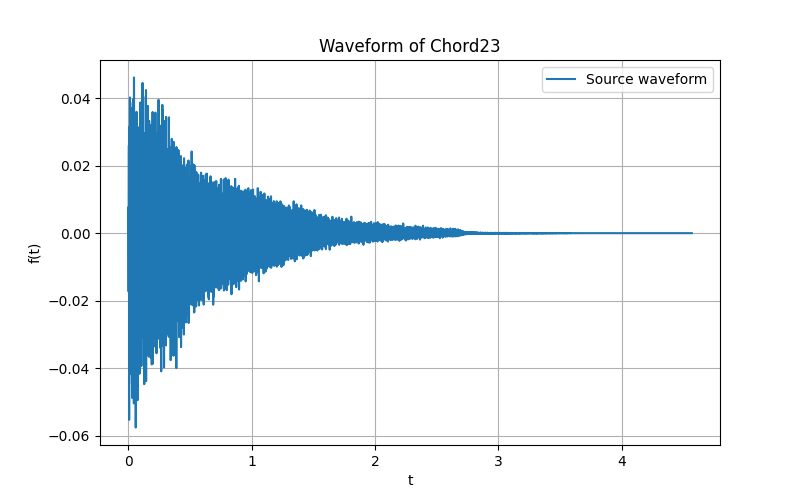
\includegraphics[width=\textwidth]{media/waveform.png}
    \caption{График зависимости уровня громкости от времени для исходной записи}
    \label{fig:waveform}
\end{figure}

Данный график обрезан по времени до 2 секунд, так как далее уровень громкости практически не изменяется.

\subsubsection{Фурье преобразование}
Теперь посмотрим на график образа данной записи в частотной области. Для этого применим к исходной записи преобразование Фурье. График зависимости уровня громкости от частоты представлен на рисунке~\ref{fig:wave_image}.

\begin{figure}[ht!]
    \centering
    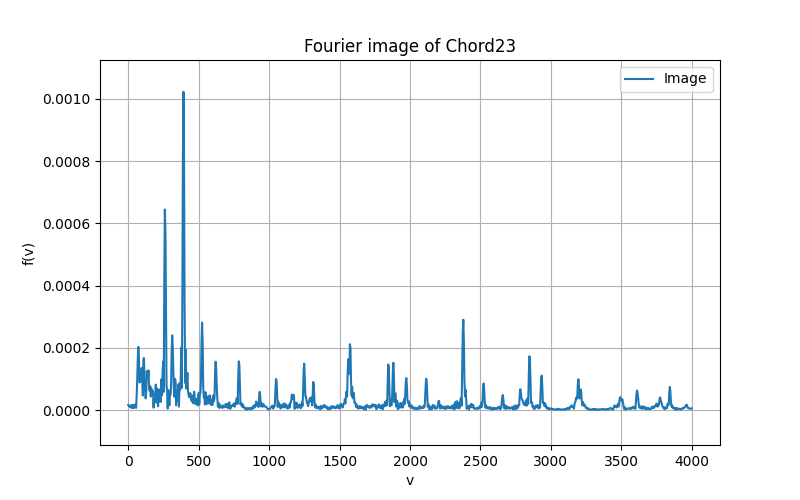
\includegraphics[width=\textwidth]{media/wave_image.png}
    \caption{График зависимости уровня громкости от частоты для исходной записи}
    \label{fig:wave_image}
\end{figure}

Для Нахождения образа использовались первые 0.1 секунда записи для того, чтобы график был более наглядным. На графики представлены частоты от 0 до 4000 Гц. 

\subsubsection{Анализ звуков}
На графике \ref{fig:wave_image} заметны явные пики, которые соответствуют доминирующим частотам. Наиболее выраженные пики находятся на частотах 262 Гц, 311 Гц и 392 Гц, что соответствует нотам C, D\# и G соответственно. Таким образом, исходный аккорд -- \textbf{До минор}. 